\documentclass{beamer}
\usepackage{../../shared/styles/custom}
\usepackage{../../shared/styles/conventions}

\usepackage{grffile}
%\beamerdefaultoverlayspecification{<+->}

\title{Lasso Regression}
\date{\today}
\author{Nipun Batra}
\institute{IIT Gandhinagar}
\begin{document}
  \maketitle

% \section{Linear Regression}

\begin{frame}random, round-robin
\item No step-size to choose!
\item Converges for Lasso objective
\end{itemize}
\end{frame}

\begin{frame}where: $$\hat{y_{i}}^{(-j)} = \theta_{0} x_{i}^{0}+\ldots + \theta_{d} x_{i}^{d}$$ is $\hat{y}_{i}$ without $\theta_{j}$
\end{frame}

\begin{frame}{Coordinate Descent for Unregularised regression}

\[
\text{Set } \frac{\partial \RSS\left(\theta_{j}\right)}{\partial \theta_{j}}= 0
\]
\[
\theta_{j}=\sum_{i=1}^{n} \frac{\left(y_{i}-\left(\theta_{0} x_{i}^{0}+\ldots + \theta_{d} x_{i}^{d}\right)\right)\left(x_{i}^{j}\right)}{\left(x_{i}^{j}\right)^{2}}= \frac{\rho_{j}}{z_{j}}
\]
\[
\rho_{j} =\sum_{i=1}^{n} x_{i}^{j}\left(y_{i}-{\hat{y}_{i}^{(-j)}}\right) \quad \text{and} \quad z_{j}=\sum_{i=1}^{n}\left(x_{i}^{j}\right)^{2}
\]
$z_{j}$ is the squared of $\ell_2$ norm of the $j^{th}$ feature
\end{frame}

%{
%\setbeamercolor{background canvas}{bg=}
%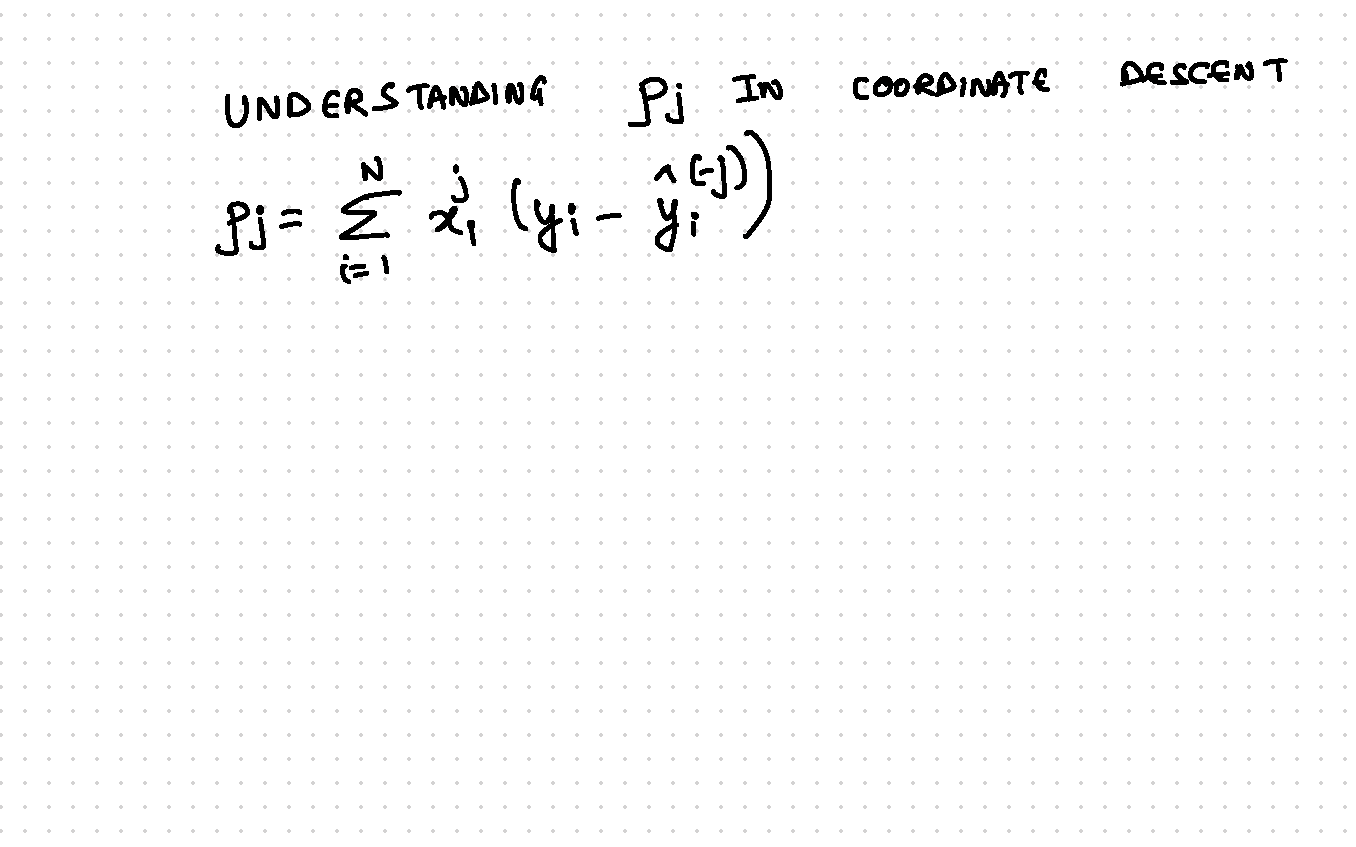
\includepdf[page=-]{coordinate-rho.pdf}
%}

\begin{frame}{Coordinate Descent for Lasso Regression}
\[
\text{Minimise} \underbrace{\sum_{i=1}^{n} \epsilon^{2} + \delta^{2}\left\{\left|\theta_{0}\right|+\left|\theta_{1}\right|+\ldots\left|\theta_{j}\right|+\ldots |\theta_{d}|\right\}}_{\text{LASSO OBJECTIVE}}
\]
\[
\frac{\partial}{\partial \theta_{j}}(\text {LASSO OBJECTIVE})=-2 \rho_{j}+2 \theta_{j} z_{j}+\delta^{2}{\frac{\partial}{\partial \theta_{j}}}\left|\theta_{j}\right|
\]
\[
\frac{\partial}{\partial \theta_{j}}\left|\theta_{j}\right|=\left\{\begin{array}{cc}
1 & \theta_{j}>0 \\
{[-1,1]} & \theta_{j}=0 \\
-1 & \theta_{j}<0
\end{array}\right.
\]
\end{frame}

\begin{frame}{Coordinate Descent for Lasso Regression}
\begin{itemize}
\item \textbf{Case 1: $\theta_{j}>0$}
\[
-2\rho_j+2\theta_j z_j+\delta^{2}  = 0
\]
\[
\theta_j = \frac{\rho_j - \frac{\delta^{2}}{2}}{z_{j}}
\]
\[
\rho_{j}>\frac{\delta^{2}}{2} \Rightarrow  \theta_{j} = \frac{\rho_j - \frac{\delta^{2}}{2}}{z_{j}}
\]

\pause
\item \textbf{Case 2: $\theta_{j}<0$}
\begin{equation}
\rho_{j} < \frac{\delta^{2}}{2} \Rightarrow \theta_{j} = \frac{\rho_{j}+\delta^{2} / 2}{z_{j}}
\end{equation}
\end{itemize}

\end{frame}

\begin{frame}{Coordinate Descent for Lasso Regression}
\begin{itemize}
\item \textbf{Case 3: $\theta_{j} = 0$}
\[
\frac{\partial}{\partial \theta_{j}}(\text {LASSO OBJECTIVE})=-2 \rho_{j}+2\theta_{j} z_{j}+ \delta^{2}\underbrace{{\frac{\partial}{\partial \theta_{j}}}\left|\theta_{j}\right|}_{\text{[-1,1]}}
\]
\[
\in \underbrace{[-2\rho_{j} - \delta^{2}, -2\rho_{j} + \delta^{2}]}_{\text{$\{0\}$ lies in this range}}
\]
\[
-2\rho_{j} - \delta^{2} \leq 0 \text{ and } -2\rho_{j} + \delta^{2} \geq 0
\]
\[
-\frac{\delta^{2}}{2} \leq \rho_j \leq \frac{\delta^{2}}{2}  \Rightarrow \theta_{j}=0
\]

\end{itemize}

\end{frame}
\begin{frame}{Summary of Lasso Regression}
\begin{equation}
\theta_{j} =\left[\begin{array}{ccc}
\frac{\rho_{j} + \frac{\delta^{2}}{2}}{z_{j}} & \text{if}  & \rho_{j}<-\frac{\delta^{2}}{2} \\
0 & \text{if} & -\frac{\delta^{2}}{2} \leq \rho_{j} \leq \frac{\delta^{2}}{2} \\
\frac{\rho_{j} - \frac{\delta^{2}}{2}}{z_{j}} & \text{if} & \rho_{j}>\frac{\delta^{2}}{2}
\end{array}\right]
\end{equation}

\end{frame}

%{
%\setbeamercolor{background canvas}{bg=}
%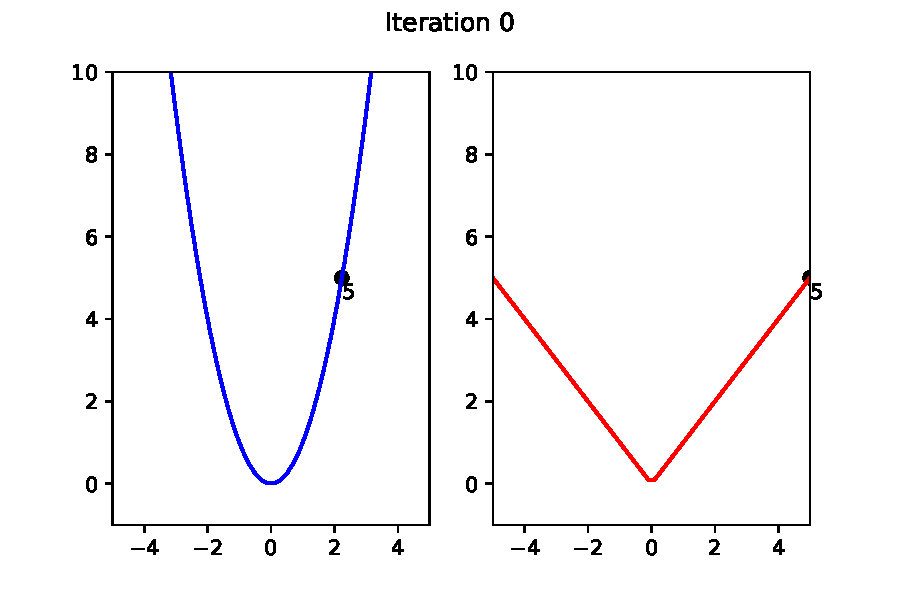
\includepdf[page=-]{coordinate-thresholding.pdf}
%}

\end{document}
